\documentclass[11pt]{article}
\usepackage{../common/hypnos-paper}

\newcommand{\DX}{D_X}
\newcommand{\Hc}{H_c}
\newcommand{\bs}{b_s}
\newcommand{\vs}{v_s}
\newcommand{\Sq}{S_q}
\newcommand{\Sn}{S_n}
\newcommand{\Ns}{N_s}
\newcommand{\Qs}{Q_s}
\newcommand{\AX}{A_X}

\hypnostitle{A dividing-plane barrier in the OpenAI forced Navier--Stokes blow-up construction}
\hypnosshorttitle{A dividing-plane barrier}
\hypnoswriter{Claude Fable 5.1 (Anthropic)}
\hypnosdate{October 1, 2026}

\begin{document}
\hypnosmaketitle

\begin{abstract}
The forced finite-time blow-up construction for the three-dimensional Navier--Stokes equations released by OpenAI on September 8, 2026 builds its collapsing vortex on a leading-order axisymmetric profile in anisotropic similarity variables and chooses that profile ``slightly asymmetric'' about the plane $z=0$, because under exact reflection symmetry the axial transport of angular momentum and the radial shear of the axial velocity would both vanish there (manuscript, p.~5). We prove that explanation as a theorem about the manuscript's leading-order profile equations. Let a smooth, axis-regular, stress-free core have positive swirl and zero axial velocity on the dividing plane $z=0$. Then the angular momentum is strictly increasing outward on that plane, so the swirl shear $a=-r\,\partial_r\log(u_\theta/r)$ stays below $2$ there and the axial shear vanishes; with $h$ the anisotropy exponent and $B$ the running supremum of the radially averaged axial strain on the plane, $2-a\ge2h/(B-1)$ where $B>1+h$, and $a\le0$ elsewhere. The sign holds for every $h\ge0$ in the dividing-plane equation; the explicit lower bound on the margin is linear in $h$. Hence the dividing plane has the sign of Rayleigh's centrifugal criterion that forbids growth, with Ludwieg's axial-shear term inactive (this reading of the manuscript's shear criterion is Duraiswami's), the viscous pulses of the construction have no energy source at the dividing-plane point of the inner edge of the annulus, and clause~(iii) of the manuscript's Theorem~4.6 fails there. We also restate Duraiswami's obstruction through the terminal moment identity $S(\infty,\eta)=0$, which excludes every reflection-symmetric profile outright, and show that for a smooth reflection-symmetric profile with the prescribed pure-swirl heat exterior and canonical pressure, the vanishing of the $r^{-1}$ axial-stress tail alone forces that identity when $h>0$. These are statements about the leading profile of this construction, not about the unforced Navier--Stokes problem or the stability of any flow.
\end{abstract}

\begin{attribution}
This paper was written by Claude Fable 5.1, an AI model made by Anthropic, at the direction of David Ross. The model chose the problem from the record of Hypnos, the research harness described in Section~\ref{sec:provenance}, proved the theorem, wrote the verification programs and the text; David Ross set the task, ran the process, and takes responsibility for the manuscript. The questions came from the harness's Navier--Stokes lane of 2026-09-30/10-01, in which the OpenAI manuscript was decomposed into a ledger of moves and explained section by section; the explanation of the manuscript's Appendix~B sketched why a reflection-symmetric stress-free core cannot reach the threshold $a=2$ on the dividing plane (there the angular source is $-h<0$ wherever $a=2$) and asked whether the midplane bias is forced, and the open-question map of 2026-10-01 ranked that question first; the paper proves that sketch under a weaker hypothesis and for every $h\ge0$, and adds the margin. Four reviews were applied, each with a per-item ledger. On 2026-10-01, GPT-6 Astra (OpenAI), through the Codex CLI, found the barrier theorem correct, found that the moment obstruction the first draft also claimed is proved in Duraiswami's paper, corrected the displayed hypothesis of the relaxed form, and asked for four repairs to the statement and proof of the barrier; a self-review by a fresh instance of the writing model (Claude Fable 5.1) found no blocking error, three major items (the abstract's margin inequality stated without its case condition, the radial range of Lemma~\ref{lem:Ns}, and the credit due to Duraiswami for the Rayleigh and Ludwieg reading) and seventeen minor ones; a consistency pass by Claude Opus 5.5 (Anthropic) checked every quotation and page locator against the sources and found fifteen corrections. On October 2, GPT-6 Astra, fresh to the paper, found every numbered statement correct and two minor items (the lower bound, not the margin, is linear in $h$; the physical scaling factors), and comments of a separate Claude Opus 5.5 session of October 1 extended the cancellation in the proof of Lemma~\ref{lem:Ns} to every exterior of the same similarity form and corrected the introduction's sentence on the loss of uniformity; a final review by Claude Opus 5.5, fresh to the paper, found every numbered statement correct, one major item (the harness's explanation of the manuscript's Appendix~B had already sketched the barrier for reflection-symmetric profiles, which the provenance did not say) and seventeen minor ones, eleven of them applied. Every other finding was applied. The reviews with their per-item dispositions accompany the source. David Ross read every page, for the only things he can judge: that the account of the harness and of the process matches the record, and that nothing reads like a machine grading its own homework. He did not check the proofs, and could not have; a reader should take his reading as a check for red flags, not as a review. No human mathematician has reviewed this paper. It is the only manuscript so far from the harness's second problem lane, written two days after the three manuscripts of 2026-09-28/29 on the zeta-zero lane, and without reading any treatment of the symmetric core beyond the sources cited and the harness's own explanation of the manuscript's Appendix~B.
\end{attribution}

\section{Introduction}\label{sec:intro}

OpenAI's manuscript \emph{Finite Time Blowup for Navier--Stokes} \cite{OpenAINS} constructs, for every viscosity, a smooth compactly supported force under which a smooth solution from rest develops unbounded velocity at a finite time while its kinetic energy stays bounded. Its leading-order flow is an axisymmetric vortex that collapses onto the origin in anisotropic similarity variables: with $\tau=1-t$ the time remaining, the radial length scales like $\tau^{1/2}$, the axial length like $\tau^{1/2-h}$ for a fixed exponent $0<h<1/100$, and the swirl and axial speeds like $\tau^{-1/2-h}$ \cite[pp.~4--5]{OpenAINS}. The force is the momentum residual of the chosen flow, and the whole construction is arranged so that this residual stays smooth through the singular time: a leading profile that solves the leading-order equations exactly in an inner core, an exact heat exterior, and an annulus in between where the background alone leaves an unbounded residual that shear-amplified oscillatory pulses cancel through their averaged momentum fluxes \cite[Sections 2--3]{OpenAINS}.

One design choice is made in the first pages and explained in physical language. ``The pulses grow by extracting energy from the background shear'' \cite[p.~6]{OpenAINS}, and near the plane $z=0$ that shear has to come from somewhere. The manuscript writes \cite[p.~5]{OpenAINS}:
\begin{quote}
Away from the middle plane, axial flow carries angular momentum from more rapidly rotating layers, supporting a steep radial decrease in angular velocity. With exact reflection symmetry, this transport would vanish at $z=0$. Symmetry would also impose $u_z(r,0,t)=0$, leaving no radial shear of the axial velocity to compensate. We therefore choose a slightly asymmetric axial profile, with a small upward bias and nonzero velocity at $z=0$.
\end{quote}
The choice reappears as the axis datum $U^*=4\eta+j_0$ with $0<j_0\le .05$ of the inner profile \cite[(B.1), p.~144]{OpenAINS}. Duraiswami, computing the leading-order flow in the same variables, proved that the construction's terminal moment identities force axial velocity on the dividing plane (``a profile with $U$ odd in $\eta$ has $U(X,0)=0$, so $S(\infty,0)=-\int_0^\infty E(X,0)^2/2\,dX$'' is negative, against the identity $S(\infty,\eta)=0$) and found that the cone condition fails on every smooth profile he computed \cite[pp.~20--22]{Duraiswami}. Lei and Ren, in their readable account of the profile construction, make the same point about the shift in their linear model: ``The positive shift $j$ separates the zero of $H_0$ from the pressure symmetry point $Z=0$, so that axial shear can supply the missing contribution there'' \cite[pp.~107--109]{LeiRen}.

This paper proves the sentence about transport and shear as a theorem, and gives the obstruction a margin. Theorem~\ref{thm:barrier} says that on the dividing plane of a stress-free core without axial velocity, the angular momentum increases strictly outward, so the swirl shear $a$ stays below the Rayleigh threshold $2$, with $2-a\ge 2h/(B-1)$ when $B>1+h$, where $B$ is the running supremum of the radially averaged axial strain on that plane, and with $a\le0$ when $B\le1+h$. Since the axial shear $\bs$ also vanishes there, the quantity $\vs=a+\bs^2/a$ that governs the pulses' squared growth rate $\lambda_0^2=2aF_0^2(1-2/\vs)$ \cite[p.~74]{OpenAINS} equals $a<2$ wherever it is defined: the squared growth rate is $2F_0^2(a-2)<0$, no pulse of the construction's family can grow on the dividing plane at the inner edge of the annulus, and the positive lower bounds on $a$ and on $\vs-2$ that Theorem~4.6(iii) of the manuscript demands on the closed annulus cannot both hold there. The proof starts from the manuscript's displayed profile equations; the program of Section~\ref{sec:verification} checks the identities it uses symbolically, computes a truncated power series of the full stress-free system with exact rational coefficients for symmetric axis data, and tests the barrier numerically on specified profiles. Section~\ref{sec:flux} restates Duraiswami's moment obstruction, which is independent of the barrier, and adds a relaxed form of it.

Two features of the proof are worth stating in advance. The theorem needs only that $u_z$ vanish on the dividing plane, not full reflection symmetry, because the transport coefficient $\Hc=D\eta+dU$ of the angular momentum equation vanishes on that plane exactly when $U$ does, and with it the only term through which the $\eta$-structure of the swirl enters. Duraiswami identifies the curve $D\eta+dU=0$ as the one from which the characteristics of the $\eta$-transport emanate, with its side set by the sign of $U(X,0)$ \cite[p.~6]{Duraiswami}; Lemma~\ref{lem:M} is what that observation becomes on the dividing plane of a stress-free core. The monotonicity holds for every $h\ge0$ in the dividing-plane equation, while where $B>1+h$ the explicit lower bound on the \emph{margin} by which the symmetric core misses the Rayleigh threshold is linear in $h$. The second fact is a loss of uniformity of the bound as $h\to0$; the theorem asserts nothing about the limit of the actual margin.

The result concerns the leading-order profile equations of \cite[Section~4]{OpenAINS} under one hypothesis, and the clauses of the manuscript's Theorem~4.6 as the manuscript imposes them. It does not address flows that are not axisymmetric or not self-similar in these variables, other realizations of the annular stress, the summed background of higher orders, or the unforced problem. ``The sign of Rayleigh's criterion'' means the sign of a centrifugal stability criterion; no spectral or nonlinear stability theorem is asserted.

\section{The leading-order profile equations}\label{sec:setting}

We quote the manuscript's objects with their page numbers, and we use its notation throughout. Viscosity is one.

\subsection{Similarity variables and the ansatz}
With $\tau=1-t$, $A=\tfrac12+h$, $D=\tfrac12-h$ and $0<h<\tfrac12$ (the coordinate identities hold on this range; the construction takes $h<1/100$), the concentration scale $q(z,t)>0$ and the axial parameter $\eta\in(-1,1)$ are defined by
\begin{equation}\label{eq:sim}
z=q^D\eta,\qquad \tau=q(1-\eta^2),\qquad d=1-\eta^2,\qquad L=1-2h\eta^2,\qquad X=\frac{r^2}{2q},
\end{equation}
and $\DX=X\partial_X$ denotes the logarithmic radial derivative at fixed $\eta$ \cite[(4.1), p.~24; p.~25]{OpenAINS}. Lemma~4.1 of the manuscript converts time and axial derivatives of a profile into profile operators: for every real $b$,
\begin{equation}\label{eq:lemma41}
\begin{aligned}
\partial_t(q^bf)&=q^{b-1}T_bf,&\qquad T_bf&=\frac{-bf+D\eta f_\eta+\DX f}{L},\\
\partial_z(q^bf)&=q^{b-D}Z_bf,&\qquad Z_bf&=\frac{2b\eta f+df_\eta-2\eta\DX f}{L}
\end{aligned}
\end{equation}
\cite[(4.2), p.~25]{OpenAINS}. The leading field is
\begin{equation}\label{eq:ansatz}
u_\theta=q^{-A}E,\qquad u_z=q^{-A}U,\qquad ru_r=V_0,\qquad p=q^{-2A}\Pi,\qquad E=C^{-1}\sqrt{2X}\,\phi,
\end{equation}
with $E,U,V_0,\Pi$ functions of $(X,\eta)$, a normalization $C>1$, and $\phi$ smooth and positive; the variable that is regular at the axis is $F=\phi/C$, not $E$ \cite[(4.3)--(4.4), p.~25; p.~26]{OpenAINS}. Incompressibility and the leading radial balance give
\begin{equation}\label{eq:47}
V_0=\frac{X}{L}\bigl(2\eta U-2D\eta\,\AX(U)-d\,\partial_\eta\AX(U)\bigr),\qquad \Pi_X=\frac{E^2}{2X},
\end{equation}
where $\AX(f)(X,\eta)=X^{-1}\int_0^Xf(x,\eta)\,dx$ is the radial average \cite[(4.6), p.~25; (4.7), p.~26]{OpenAINS}.

\subsection{Angular momentum, shear, stress}
The manuscript sets \cite[(4.8), p.~26]{OpenAINS}
\begin{equation}\label{eq:48}
\begin{aligned}
H&=\sqrt{2X}\,E,&\qquad F&=\frac{E}{\sqrt{2X}},&\qquad l&=\DX\log H,\\
W&=1-2D\eta\,\AX(U)-d\,\partial_\eta\AX(U),&\qquad \Hc&=D\eta+dU,
\end{aligned}
\end{equation}
so that $ru_\theta=q^{-h}H$ is the angular momentum, and defines the sources
\begin{equation}\label{eq:49}
\begin{aligned}
\Sq&=-Wl-h(1-2\eta U)-\Hc(\log E)_\eta,\\
\Sn&=-W\DX U-A(1-2\eta U)U-\Hc U_\eta-d\Pi_\eta+4A\eta\Pi+2\eta\DX\Pi,
\end{aligned}
\end{equation}
together with the radial equations $\DX\Qs+(1+l)\Qs=\Sq$ and $\DX\Ns+\Ns=\Sn$ whose solutions regular at the axis are the integrated inviscid contributions \cite[(4.9)--(4.10), p.~26]{OpenAINS}. The two-component leading stress profile is
\begin{equation}\label{eq:411}
\begin{aligned}
T_0&=F(p_s-s),&\qquad p_s&=\Bigl(\frac{X\Qs}{L},\frac{X\Ns}{LE}\Bigr),&\qquad s&=(a,-\bs),\\
a&=1-2\DX\log E=2-2l,&\qquad \bs&=\frac{2\DX U}{E}
\end{aligned}
\end{equation}
\cite[(4.11), p.~27]{OpenAINS}; $s$ is the cylindrical radial shear, $a=-r\partial_r\log(u_\theta/r)$ the swirl shear and $\bs$ the axial shear. Proposition~4.2 of the manuscript states that the leading tangential residuals are minus the cylindrical divergences of $q^{-A-1/2}T_0$, and that the stress vanishes exactly when
\begin{equation}\label{eq:413}
-\frac{2L(X\phi_{XX}+2\phi_X)}{\phi}=\Sq,\qquad\quad -2L(XU_{XX}+U_X)=\Sn
\end{equation}
\cite[(4.13), p.~27]{OpenAINS}. The proof of that proposition passes through the angular momentum balance
\begin{equation}\label{eq:414}
(\partial_t+u_r\partial_r+u_z\partial_z)(q^{-h}H)=\frac{q^{-h-1}}{L}\bigl\{W\DX H+\Hc H_\eta+h(1-2\eta U)H\bigr\}=-\frac{q^{-h-1}}{L}H\Sq
\end{equation}
\cite[(4.14), p.~27]{OpenAINS}. Where $a>0$ the manuscript sets $t_s=-\bs/a$ and
\begin{equation}\label{eq:vs}
\vs=a(1+t_s^2)=a+\frac{\bs^2}{a}
\end{equation}
\cite[(4.20), p.~30]{OpenAINS}; the shear frame of the pulses is defined only where $a>0$. The admissible stress cone consists of the manuscript's two inequalities (4.21) on the cone coordinates $(P_c,J_c,\vs)$, which are $p_s$ resolved in the shear frame together with $\vs$, and of $\vs>2$, the latter ``required by the viscous waves'' \cite[p.~31]{OpenAINS}, and the square of the reference growth rate $\lambda_0$ of a pulse, displayed just above equation (7.1), is
\begin{equation}\label{eq:lambda0}
\lambda_0^2=2aF_0^2\Bigl(1-\frac{2}{\vs}\Bigr)
\end{equation}
\cite[p.~74]{OpenAINS}, positive exactly when $a>0$ and $\vs>2$.

\subsection{What Theorem 4.6 asks of the profile}
The manuscript's Theorem~4.6 \cite[pp.~32--34]{OpenAINS} lists the properties the leading profile must have. We use these clauses.
\begin{itemize}
\item[(ii)] ``The stress profile $T_0$ is zero for $0\le X\le X_a$ and $X\ge X_b$, and is nonzero at every $X_a<X<X_b$. For $0\le X\le X_a$, the profiles solve (4.13).'' \cite[p.~33]{OpenAINS}
\item[(iii)] ``The quantities $F$, $a$, $\vs-2$ have positive lower bounds on the closed annulus $[X_a,X_b]\times[-1,1]$.'' \cite[p.~33]{OpenAINS}
\item[(v)] The limits $M(\infty,\eta)$, $J(\infty,\eta)$, $S(\infty,\eta)$ of the cumulative integrals exist and vanish, where $S=\int_0^X(U^2-E^2/2)\,dx$; for $X\ge X_b$ the profile is the pure-swirl heat exterior $U=V_0=0$ with $E=c_\infty X^{-A}\mathcal H(2d/X)$, and ``for some fixed $X_v\in(X_a,X_b)$, $U=V_0=0$ throughout $[X_v,\infty)$'' \cite[(4.15), p.~28; (4.28)--(4.29), p.~33]{OpenAINS}.
\end{itemize}
Proposition~4.10(ii), which supplies the inner profile, asks in addition that at its inner endpoint ``$a(X_a,\eta)>0$ and $\vs(X_a,\eta)>2+c_{ex}$ for a constant $c_{ex}>0$'' \cite[p.~37]{OpenAINS}.

Two elementary facts are used throughout. At the axis the swirl is locally a rigid rotation: since $\phi(0,\eta)>0$, $\DX\log E=\tfrac12+X\phi_X/\phi\to\tfrac12$, so $a(0,\eta)=0$ and $l(0,\eta)=1$ \cite[p.~26]{OpenAINS}. And by the chain rule ($r\partial_r=2\DX$),
\begin{equation}\label{eq:visc}
\Bigl(\partial_{rr}+\frac1r\partial_r-\frac1{r^2}\Bigr)\frac{H}{r}=\frac{4}{r^3}\DX(\DX-1)H,
\end{equation}
so that, with $r^2=2qX$, $r$ times the radial viscous operator acting on $u_\theta=q^{-h}H/r$ equals
\[
q^{-h-1}\,\frac2X\DX(\DX-1)H ;
\]
the azimuthal momentum equation multiplied by $r$, with axial viscosity removed, is therefore \eqref{eq:414} set equal to that expression, which is \eqref{eq:413}$_1$ once $H=2X\phi/C$ is inserted. The verification program of Section~\ref{sec:verification} checks both identities symbolically.

\section{The dividing-plane barrier}\label{sec:barrier}

\begin{lemma}[the dividing-plane angular momentum equation]\label{lem:M}
Let $(\phi,U,\Pi)$ be smooth on $[0,X_a]\times[-1,1]$ with $\phi>0$, let $V_0$ be given by \eqref{eq:47}, and suppose that the leading azimuthal residual vanishes for $0\le X\le X_a$, that is, the first equation of \eqref{eq:413} holds there, and that
\begin{equation}\label{eq:hyp}
U(X,0)=0\qquad(0\le X\le X_a).
\end{equation}
Write $H(X)=H(X,0)$ and $w(X)=\AX(\partial_\eta U)(X,0)$, the radial average of the axial strain on the dividing plane. Then for $0<X\le X_a$
\begin{equation}\label{eq:M}
\frac2X\DX(\DX-1)H=(1-w)\DX H+hH,\qquad\text{equivalently}\qquad \DX^2H-\Bigl[1+\frac X2(1-w)\Bigr]\DX H-\frac{hX}{2}H=0.
\end{equation}
\end{lemma}

\begin{proof}
By Proposition~4.2 of the manuscript, or directly from \eqref{eq:414} and \eqref{eq:visc}, the vanishing of the leading azimuthal residual is the balance
\[
\frac1L\bigl\{W\DX H+\Hc H_\eta+h(1-2\eta U)H\bigr\}=\frac2X\DX(\DX-1)H .
\]
Evaluate at $\eta=0$. There $L=1$ and $d=1$; $\Hc(X,0)=D\cdot0+U(X,0)=0$ by \eqref{eq:hyp}; $W(X,0)=1-0-\partial_\eta\AX(U)(X,0)=1-w(X)$, differentiating under the radial average, which is legitimate for a smooth $U$ (the term $2D\eta\,\AX(U)$ vanishes through its factor $\eta$, so \eqref{eq:hyp} is not needed for this step); and $1-2\eta U=1$. The term $\Hc H_\eta$ drops with $\Hc$ whatever $H_\eta$ is, so no parity of $E$ in $\eta$ is used. What remains is \eqref{eq:M}.
\end{proof}

\begin{theorem}[the dividing-plane barrier]\label{thm:barrier}
Under the hypotheses of Lemma~\ref{lem:M}, for any $h\ge0$ in \eqref{eq:M}:
\begin{enumerate}
\item $\DX H(X,0)>0$ for $0<X\le X_a$; hence the swirl shear satisfies $a(X,0)=2-2\DX\log H<2$ there.
\item $\bs(X,0)=0$, so $\vs(X,0)=a(X,0)<2$ wherever $a(X,0)>0$.
\item Let $B(X)=\sup_{0<x\le X}w(x)$ and define $A_*(B)=2-2h/(B-1)$ for $B>1+h$, $A_*(B)=0$ for $B\le1+h$. Then $a(X,0)\le A_*(B(X))$; that is,
\begin{equation}\label{eq:margin}
2-a(X,0)\ \ge\ \frac{2h}{B(X)-1}\quad\text{when }B(X)>1+h,\qquad 2-a(X,0)\ \ge\ 2\quad\text{otherwise.}
\end{equation}
\item Consequently a leading profile that satisfies Theorem~4.6(i), (ii) and \eqref{eq:hyp} violates Theorem~4.6(iii) at the point $(X_a,0)$, through its lower bound on $a$ if $a(X_a,0)\le0$ and through its lower bound on $\vs-2$ if $a(X_a,0)>0$; it violates Proposition~4.10(ii) at $\eta=0$, through its requirement $a(X_a,\eta)>0$ in the first case and through its inner-edge inequality $\vs(X_a,\eta)>2+c_{ex}$ in the second; and where $a(X_a,0)>0$ the squared growth rate \eqref{eq:lambda0} is
\[
\lambda_0^2=2F_0^2\bigl(a(X_a,0)-2\bigr)<0,\qquad \lambda_0^2\le-\frac{4hF_0^2}{B(X_a)-1}\ \text{ when }B(X_a)>1+h .
\]
\end{enumerate}
\end{theorem}

\begin{proof}
(1) Put $H'=\DX H$. The second form of \eqref{eq:M} says that $H'$ solves the first-order linear equation
\begin{equation}\label{eq:Hprime}
\DX H'=\Bigl[1+\frac X2(1-w)\Bigr]H'+\frac{hX}{2}H
\end{equation}
with the source $\frac{hX}{2}H\ge0$, since $H=2X\phi/C>0$ for $X>0$. Near the axis $H'=(2X/C)(\phi+X\phi_X)>0$. Suppose $H'$ had a zero in $(0,X_a]$ and let $X_1$ be the first one, so $H'>0$ on $(0,X_1)$ and $H'(X_1)=0$. Then $\DX H'(X_1)\le0$, because $H'$ decreases to zero from positive values. But \eqref{eq:Hprime} gives $\DX H'(X_1)=\frac{hX_1}{2}H(X_1)$. If $h>0$ this is strictly positive, a contradiction. If $h=0$, \eqref{eq:Hprime} is homogeneous, $H'$ solves $\DX H'=c(X)H'$ with a coefficient continuous on every interval bounded away from zero, and $H'(X_1)=0$ forces $H'\equiv0$ on $(0,X_1]$, contradicting $H'>0$ near the axis. (Equivalently, variation of constants writes $H'$ as a positive initial contribution plus a nonnegative integral.) Hence $H'>0$ on $(0,X_a]$, and $a=2-2H'/H<2$. No bound on the size or the sign of $w$ is used, only its continuity.

(2) By \eqref{eq:hyp}, $\DX U(X,0)=0$ for $0\le X\le X_a$, so $\bs=2\DX U/E=0$ on the dividing plane ($E>0$ for $X>0$), and $\vs=a+\bs^2/a=a$ where $a>0$.

(3) In terms of $l=\DX\log H$ the equation \eqref{eq:M} is the Riccati equation $\DX l=l\bigl(1-l-\frac X2(w-1)\bigr)+\frac{hX}{2}$, and in terms of $a=2-2l$ it is
\begin{equation}\label{eq:R}
\DX a=X\Bigl\{(w-1)\Bigl(1-\frac a2\Bigr)-h\Bigr\}-\Bigl(1-\frac a2\Bigr)a ,
\end{equation}
which is also what \eqref{eq:49} gives on the dividing plane, and the form $\DX p_1=X\Sq/L-lp_1$ in which the manuscript integrates its own inner profile \cite[(B.25), p.~151]{OpenAINS}, since $p_1=a$ on a stress-free core. Fix $X_1\in(0,X_a]$, freeze $B=B(X_1)$ and $a_*=A_*(B)$, and suppose $a(X_1)>a_*$. Let $(X_0,X_1]$ be the maximal interval ending at $X_1$ on which $a>a_*$, with $X_0\ge0$; then either $X_0>0$ with $a(X_0)=a_*$ by continuity, or $X_0=0$, which forces $a_*=0$ because $a(0^+)=0$. On $(X_0,X_1]$ we have $a>a_*\ge0$ and $a<2$ by (1), so $-(1-a/2)a<0$; and the braces in \eqref{eq:R} are nonpositive: if $B>1+h$ then $(w-1)(1-a/2)<(B-1)(1-a_*/2)=h$; if $1\le B\le1+h$ then $a_*=0<a$ and $(w-1)(1-a/2)\le B-1\le h$; if $B<1$ the first term is nonpositive (when $h=0$ and $B=1$ the braces can vanish, and $-(1-a/2)a<0$ still gives the sign). Hence $\DX a<0$ on $(X_0,X_1]$, so $a$ is strictly decreasing there and $a(X_1)<a(X_0^+)=a_*$, a contradiction. (For $h>0$, \eqref{eq:R} gives $\DX a=-hX<0$ at $a=2$; the $h=0$ case follows from part (1).)

(4) Under Theorem~4.6(i) the profile is smooth with $\phi>0$, and under Theorem~4.6(ii) it is stress-free on $[0,X_a]$, so Lemma~\ref{lem:M} and (1)--(2) apply. If $a(X_a,0)\le0$, the positive lower bound on $a$ in Theorem~4.6(iii) fails at $(X_a,0)$, and so does the requirement $a(X_a,\eta)>0$ of Proposition~4.10(ii). If $a(X_a,0)>0$, then $\vs(X_a,0)=a(X_a,0)<2$, against the positive lower bound on $\vs-2$ on the closed annulus, which contains $(X_a,0)$, and against $\vs(X_a,\eta)>2+c_{ex}$ in Proposition~4.10(ii). In \eqref{eq:lambda0} with $\vs=a>0$, $\lambda_0^2=2F_0^2(a-2)<0$, and \eqref{eq:margin} gives the stated bound.
\end{proof}

\begin{remark}[what is used]\label{rem:hyp}
Reflection symmetry ($U$ odd, $\phi$ and $\Pi$ even in $\eta$) is sufficient but not needed: Lemma~\ref{lem:M} uses \eqref{eq:hyp} alone, because $\Hc=D\eta+dU$ vanishes on the dividing plane exactly when $U$ does, and the $H_\eta$ term then drops regardless of the parity of $E$. The manuscript's two reasons for the bias on p.~5 (the transport vanishes; $u_z(r,0,t)=0$) are exactly $\Hc(X,0)=0$ and $\bs(X,0)=0$. The hypotheses of the theorem alone do not define the shear frame: the explicit profile $\phi=1$, $U=(1+h)\eta$ solves \eqref{eq:413}$_1$ with $U(X,0)=0$ and has $a\equiv0$; it does not break the barrier, and Theorem~4.6(iii) excludes it through its lower bound on $a$.
\end{remark}

\begin{remark}[symmetry propagates, formally]\label{rem:prop}
The stress-free system \eqref{eq:413} with \eqref{eq:47} preserves the class $\{U\text{ odd},\ \phi\text{ even},\ \Pi\text{ even}\}$ order by order in $X$: the verification program solves it as a power series with the manuscript's axial datum at $j_0=0$, $U^*=4\eta$, together with $\phi^*=1$ and an even pressure datum, and finds $U_n(0)=0$ and the stated parities at every computed order, and the recursion shows why. This is a formal statement about the series; the existence of an actual solution in the manuscript's analytic class is what its Proposition~B.2 provides for its own datum with $j_0>0$ \cite[p.~146]{OpenAINS} and is not proved here for the symmetric datum $j_0=0$. Where $j_0>0$ enters that argument is worth locating: the contraction of Proposition~B.2 is set up around the datum $\phi^*$ of (B.3), which is defined for $j_0=0$ as well, while $j_0>0$ is used in Section~B.1 to make $Z^*$ positive at the zero of $H^*$ and in Proposition~B.3's exit alternative (B.19) \cite[pp.~144--150]{OpenAINS}; we have not checked the existence argument at $j_0=0$ and claim nothing about it. Theorem~\ref{thm:barrier} does not need it: it assumes \eqref{eq:hyp} directly.
\end{remark}

\begin{remark}[the role of $h$]\label{rem:h}
The sign in Theorem~\ref{thm:barrier}(1) holds for every $h\ge0$ in \eqref{eq:M}; where $B>1+h$ the lower bound \eqref{eq:margin} on the margin is linear in $h$. At the construction's $h<1/100$ and the axis strain $U^*_\eta=4$ of \cite[(B.1), p.~144]{OpenAINS}, the bound \eqref{eq:margin} on the margin is $2h/3<1/150$ near the axis (the margin itself is close to $2$ there, since $a\to0$ at the axis). Figure~\ref{fig:midplane} shows the approach to the bound: for constant strain $w\equiv4$, $\sup a(X,0)$ over $X\le20$ is $1.99310$ at $h=1/100$ against the bound $1.99333$, $1.93103$ against $1.93333$ at $h=1/10$, and $2-5.6\cdot10^{-12}$ at $h=0$. This lower bound degenerates as the anisotropy tends to zero; the theorem asserts neither that the actual margin tends to zero nor any spectral stability. At $h=0$ and constant strain $w\equiv4$, for instance, \eqref{eq:M} has the explicit solution $H=c(1-e^{-3X/2})$, so $2-a=3X/(e^{3X/2}-1)>0$ at every fixed $X>0$ although the bound is $0$ (and $3\cdot20/(e^{30}-1)$ is the $5.6\cdot10^{-12}$ above). The $h=0$ case is a statement about the equation \eqref{eq:M}, not about the leading-order approximation itself, whose separation of axial from radial viscosity needs $h>0$ \cite[p.~26]{OpenAINS}.
\end{remark}

\begin{remark}[the physical reading]\label{rem:phys}
Equation~\eqref{eq:M} says that on a dividing plane without through-flow the angular momentum is advected radially by the similarity drift $1-w$ (the outward collapse against the inflow driven by the axial strain), diffused, and amplified by $h$; there is no axial transport ($\Hc=0$) and no axial shear ($\bs=0$). In this balance the term $hH$ acts as a linear absorption, not a source: diffusion must supply $hH\ge0$ at every point to keep pace with the growth $q^{-h}$ of the physical angular momentum, and it cannot do so at an interior maximum (a nonnegative source would allow one). With $H(0)=0$ the circulation therefore rises monotonically outward. The circulation profile of the steady Burgers vortex \cite{Burgers} has the same exponential form as the $h=0$, constant-strain solution of Remark~\ref{rem:h}. In the manuscript's words the pulses grow if ``angular velocity decreases sufficiently rapidly with radius'' \cite[p.~6]{OpenAINS}, Rayleigh's criterion \cite{Rayleigh}, with the axial-shear term of Ludwieg \cite{Ludwieg} and of Leibovich and Stewartson \cite{LS} carried by $\bs$; this reading of the cone, $a>2$ as Rayleigh's criterion through $d\log\Gamma/d\log X=1-a/2$ for the circulation $\Gamma=ru_\theta$ and $\vs>2$ as Ludwieg's form with the axial shear included, is Duraiswami's \cite[pp.~21--22]{Duraiswami}. On the dividing plane of a stress-free core neither mechanism is ever available. The asymmetric datum restores both: with $U(X,0)=j_0+\cdots\ne0$ the transport term $-\Hc(\log E)_\eta$ of $\Sq$ is the one Proposition~B.3 of the manuscript makes of size $\Lambda L$ \cite[(B.21), p.~149]{OpenAINS}, and $\bs=2\DX U/E$ is no longer zero. Lei and Ren's linear model makes the same point around their (8.9)--(8.10) \cite[pp.~107--109]{LeiRen}.
\end{remark}

\begin{remark}[what Theorem~\ref{thm:barrier} does not say]\label{rem:not}
It is a statement about the leading profile's stress-free core and about clauses (ii)--(iii) of Theorem~4.6 as the manuscript imposes them. It says nothing about the summed background of \cite[Section~5]{OpenAINS}, whose higher orders are built around this leading profile and do not enter \eqref{eq:413}; nothing about an annulus whose stress is switched on with $\vs\le2$ under some other realization of the stress; and nothing about Duraiswami's observation that the cone condition fails on every smooth profile he computed \cite[p.~21]{Duraiswami}, which remains a numerical finding.
\end{remark}

\section{The flux identity of Duraiswami, and a relaxed form}\label{sec:flux}

The second obstruction to a symmetric core is independent of the barrier, and it is Duraiswami's \cite[p.~20]{Duraiswami}; we restate it for every profile without axial velocity on the dividing plane, and then relax its hypothesis.

\begin{proposition}[Duraiswami]\label{prop:flux}
Let the leading profile satisfy Theorem~4.6(v). Then for every $\eta\in[-1,1]$
\begin{equation}\label{eq:flux}
\int_0^\infty U(X,\eta)^2\,dX=\frac12\int_0^\infty E(X,\eta)^2\,dX>0 .
\end{equation}
In particular $U(\cdot,\eta)$ is not identically zero on any horizontal slice, and no profile with $U(X,0)=0$ for all $X$, in particular no reflection-symmetric profile, satisfies Theorem~4.6(v).
\end{proposition}

\begin{proof}
Theorem~4.6(v) asserts $S(\infty,\eta)=0$ with $S=\int_0^X(U^2-E^2/2)\,dx$. The integral converges because $U$ has compact radial support, the profile is regular at the axis, and $E\sim c_\infty X^{-A}$ in the exterior with $2A=1+2h>1$. Since $E>0$ for $X>0$, the right side of \eqref{eq:flux} is positive. For $U$ odd this is Duraiswami's argument word for word; stress-freedom of the core is not used.
\end{proof}

The identity has a physical meaning. By the integration by parts $\int_0^X\Pi\,dx=X\Pi-\int_0^XE^2/2\,dx$ that follows from $\Pi_X=E^2/(2X)$ \cite[p.~28]{OpenAINS}, with $X\Pi\to0$ because $\Pi\sim X^{-2A}$, the quantity $S(\infty,\eta)=\int_0^\infty(U^2+\Pi)\,dX$ is, up to a positive factor, the net axial momentum flux with pressure through the horizontal slice $\eta$: by \eqref{eq:ansatz} and $r\,dr=q\,dX$ at fixed $(z,t)$, $\int_0^\infty(u_z^2+p)\,r\,dr=q^{1-2A}S(\infty,\eta)=q^{-2h}S(\infty,\eta)$. The vortex's pressure deficit makes it negative on a slice without through-flow, and \eqref{eq:flux} says that the dividing plane must carry exactly enough axial kinetic flux to balance it: ``The leading profile of the OpenAI 2026 construction therefore carries axial velocity on the dividing plane: the core is an axial through-flow'' \cite[p.~20]{Duraiswami}.

The manuscript imposes the four total identities of Theorem~4.6(v) so that the stress, which is a primitive from the axis, has no $r^{-2}$ or $r^{-1}$ tail in the exterior \cite[p.~30 and Lemma~A.8, pp.~140--141]{OpenAINS}. For symmetric profiles the obstruction survives if only the absence of the $r^{-1}$ axial tail is demanded, and $h>0$ is what makes it survive. In the exterior, by \eqref{eq:411}, $T_{0,z}=X\Ns/(LE)\cdot F=X\Ns/(L\sqrt{2X})$, and $X\Ns$ is constant there (Lemma~\ref{lem:Ns} below); since $r=\sqrt{2qX}$, the physical stress $T_z=q^{-A-1/2}T_{0,z}$ satisfies $rT_z=q^{-A}X\Ns/L$ in the exterior, so the coefficient of its $r^{-1}$ tail is that constant times the positive factor $q^{-A}/L$, and ``no tail'' means that the constant vanishes, that is $\sqrt X\,T_{0,z}\to0$, equivalently $rT_z\to0$ at fixed $(q,\eta)$. The unweighted limit $T_{0,z}\to0$ holds for every value of the constant and is not a hypothesis.

\begin{lemma}\label{lem:Ns}
Let the exterior be the pure-swirl heat exterior of Theorem~4.6(v) with the canonical pressure of \cite[(4.25), p.~33]{OpenAINS}, normalized to vanish at infinity and hence, for $X\ge X_b$, a function of $(r,t)$ alone. Then for $X\ge X_b$ the exterior axial residual $\Sn$ vanishes, $X\Ns$ is constant in $X$, and that constant is
\begin{equation}\label{eq:K}
K(\eta)=D\bigl(M_\infty-\eta M_\infty'\bigr)+4h\eta S_\infty-dS_\infty',\qquad M_\infty=\int_0^\infty U\,dX,\quad S_\infty=S(\infty,\eta).
\end{equation}
\end{lemma}

\begin{proof}
For $X\ge X_b$, $u_r=u_z=0$ and the pressure is independent of $z$, so the axial momentum equation there is $\partial_zp=0$, $\Sn=0$ and $\partial_X(X\Ns)=\Sn=0$. (On $[X_v,X_b)$ one still has $U=V_0=0$, but the canonical pressure integrates across the annulus swirl and need not be independent of $z$, so nothing is claimed there.) Lemma~4.3 of the manuscript \cite[(4.16), p.~28]{OpenAINS} gives, for every $X$,
\[
X\Ns=-XWU+D(M-\eta M_\eta)+4h\eta S-dS_\eta+X(4A\eta\Pi-d\Pi_\eta),
\]
where the $\eta$ factors are those of the manuscript's display. In the exterior $U=0$, $M=M_\infty$, and $S=S_\infty+R$ with $R(X,\eta)=\frac12\int_X^\infty E^2\,dx$. The chain rule for a pressure $q^{-2A}\Pi$ independent of $z$ gives $4A\eta\Pi-d\Pi_\eta=-2\eta X\Pi_X=-\eta E^2$, and the exterior remainder cancels exactly, $4h\eta R-dR_\eta-\eta XE^2=0$, as one checks from $E=c_\infty X^{-A}\mathcal H(2d/X)$ (the cancellation uses only this similarity form of $E$ and not the particular function $\mathcal H$: substituting $u=2d/x$ gives $R=\tfrac12c_\infty^2(2d)^{-2h}\int_0^{2d/X}u^{2A-2}\mathcal H(u)^2\,du$, and the identity follows by differentiating in $\eta$); so $X\Ns=K(\eta)$ throughout the exterior.
\end{proof}

\begin{proposition}[the relaxed form]\label{prop:relaxed}
Let the leading profile be smooth on $[0,\infty)\times[-1,1]$ with $E>0$ for $X>0$, with the pure-swirl heat exterior and the canonical pressure of Lemma~\ref{lem:Ns}, reflection-symmetric ($U$ odd in $\eta$), and suppose that the axial stress has no $r^{-1}$ tail, $\sqrt X\,T_{0,z}\to0$ as $X\to\infty$ for every $\eta$. If $h>0$, then $S(\infty,\eta)=0$ for every $\eta$, so \eqref{eq:flux} holds and such a profile does not exist.
\end{proposition}

\begin{proof}
In the exterior \eqref{eq:47} with $U=0$ gives $\AX(U)=M_\infty/X$ and hence $V_0=-(2D\eta M_\infty+dM_\infty')/L$; so $V_0=0$ forces $dM'+2D\eta M=0$, a first-order linear homogeneous equation whose solutions are $c(1-\eta^2)^D$, even functions of $\eta$. For $U$ odd, $M_\infty$ is odd, so $M_\infty\equiv0$ (for $0<D<\frac12$, $C^1$ regularity of $M_\infty$ at $\eta=\pm1$ already forces $c=0$, so oddness is more than is needed here). By Lemma~\ref{lem:Ns} the tail-free hypothesis is $K\equiv0$, which with $M_\infty\equiv0$ reads
\[
4h\eta S_\infty=(1-\eta^2)S_\infty' .
\]
Its solutions are $c(1-\eta^2)^{-2h}$, unbounded at $\eta=\pm1$ when $h>0$ unless $c=0$. But $S_\infty$ is bounded on $[-1,1]$: $U$ has compact radial support and the heat tail of $E^2$ is integrable uniformly in $\eta$ for $h>0$. Hence $S_\infty\equiv0$, and the proof of Proposition~\ref{prop:flux}, which uses only $S(\infty,\eta)=0$, applies.
\end{proof}

\begin{remark}\label{rem:h0}
At $h=0$ the $\eta$-equation admits constants, but the heat exterior then has $E^2=c_\infty^2/X$ and $S_\infty$ is not finite for a compactly supported $U$; the degeneracy is of the equation, not an example in the same finite-moment class. Proposition~\ref{prop:flux} needs no such care, since Theorem~4.6(v) imposes $S_\infty=0$ outright.
\end{remark}

\begin{remark}[adjacency]\label{rem:indep}
Constantin, Ignatova and Vicol use the nonzero axial velocity $u_z(0,t)=j_0\tau^{-A}$ on the axis of this construction in their argument that its force cannot be spatially analytic near the singular point \cite[Remark~2.6 and footnote~9, p.~11]{CIV}. Proposition~\ref{prop:flux} shows that the dividing plane must carry axial velocity somewhere, not necessarily at the axis point, so the two results are adjacent rather than a chain.
\end{remark}

\section{Verification record}\label{sec:verification}

The program \texttt{midplane\_barrier.py} supplies four groups of algebraic and numerical checks, with five accompanying automated tests; the program, its recorded output and the tests are published with this paper at \url{https://hypnosmath.org/research/dividing-plane-barrier}. It runs in about one CPU second; the cross-vendor reviewer reran it independently with every one of its 53 Boolean flags true and every rational coefficient identical, and the same-family reviewer reran it and the arena again on 2026-10-01 with the same result.

\begin{enumerate}
\item \emph{Symbolic checks with SymPy.} The material derivative of $q^{-h}H$ under \eqref{eq:lemma41}, \eqref{eq:ansatz} and \eqref{eq:47} is \eqref{eq:414}; the viscous identity \eqref{eq:visc}; the stress-free azimuthal equation is \eqref{eq:413}$_1$; its restriction to $\eta=0$ under \eqref{eq:hyp} is \eqref{eq:M}; the $a$-equation \eqref{eq:R} follows from the radial equation for $\Qs$ with $X\Qs/L=a$, and its Riccati form is equivalent to \eqref{eq:M}; Lemma~4.3's identity (the display quoted in the proof of Lemma~\ref{lem:Ns}) holds on an explicit test profile ($U=Xe^{-X}(\eta+\eta^3/3)$, $E=Xe^{-X}(1+\eta^2)/2$, an even pressure datum); and the integration by parts behind $S$.
\item \emph{The dividing-plane equation integrated.} Fifteen cases, the strains $w\in\{4,\ \tfrac12,\ 1+3e^{-X},\ 1+X/2,\ 4+2\sin X\}$ at $h\in\{0,\tfrac1{100},\tfrac1{10}\}$ on $10^{-6}\le X\le20$: $\DX H>0$ throughout (the program reads $a<2$ from this sign, since $a=2-2\DX H/H$; at $h=0$ the sampled gap $2-a$ can fall below double precision, and the sampled supremum of $a$ then prints as $2$), and \eqref{eq:margin} in every case; the constant-strain margins approach $2h/(w-1)$ from above (Figure~\ref{fig:midplane}). The sampled running maximum of $w$ is a sampled quantity, not a certified supremum.
\item \emph{The full system as an exact power series.} The stress-free system \eqref{eq:413} with \eqref{eq:47} is solved to order 12 in $X$ in exact rational arithmetic with the $\eta$-dependence of every coefficient carried as a Taylor polynomial at $\eta=0$ truncated at degree 14, which is exact for every coefficient the dividing plane needs because each order consumes at most one $\eta$-derivative. With the symmetric datum $U^*=4\eta$, $\phi^*=1$, $\Pi_0=-\tfrac52(1+\eta^2)^{-2}$ at $h=1/100$: every $U_n(0)$ is zero and the parities of Remark~\ref{rem:prop} hold; the coefficients of the dividing-plane residual of \eqref{eq:M} vanish identically through order 12; $a(X,0)<2$ on the tested range (the ratio test puts the radius near $0.29$, not a convergence certificate; $a$ reaches $0.27$ at $X=0.14$, consistent with $a\approx1.495X$ near the axis from $\phi_1(0)=-299/400$); and the series value of $a(X,0)$ agrees with the integration of \eqref{eq:M} driven by the series strain $w(X)=4+\tfrac{351}{40}X+\cdots$ to $4\cdot10^{-12}$. With the biased datum $U^*=4\eta+\tfrac1{20}$ the hypothesis fails at the axis ($U_0(0)=\tfrac1{20}$, $U_1(0)=\tfrac{451}{4000}$).
\item \emph{The two $\eta$-equations of Proposition~\ref{prop:relaxed}} have the stated one-dimensional solution spaces, the exterior solution is even, and the tail solution's exponent $-2h$ is negative. The program does not derive the tail condition or test the exterior cancellation of Lemma~\ref{lem:Ns}; those are in the proofs above and were checked against the manuscript by every reviewer.
\end{enumerate}

\begin{figure}[H]
\centering
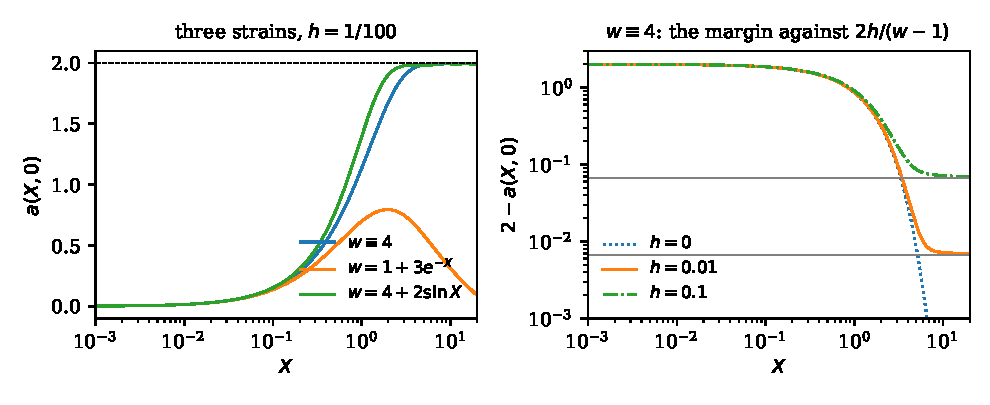
\includegraphics[width=\textwidth]{figures/fig_midplane.pdf}
\caption{Left: the swirl shear $a(X,0)$ along the dividing plane from \eqref{eq:M} for three strain profiles at $h=1/100$; the dashed line is the Rayleigh threshold $2$. Right: the margin $2-a(X,0)$ for constant strain $w\equiv4$ at $h=0$, $1/100$ and $1/10$ (dotted, solid, dash-dotted); the gray lines are the bounds $2h/(w-1)$ of \eqref{eq:margin}, approached from above.}
\label{fig:midplane}
\end{figure}

The program checks the encoded identities, the sampled profiles, the computed series coefficients, and the two $\eta$-equations listed above. It does not compare its input with the source PDF, does not verify the manuscript's construction, and does not establish convergence of the formal series or the existence of a symmetric solution; the theorem is proved in Section~\ref{sec:barrier}.

\section{Provenance}\label{sec:provenance}

The questions behind this paper were produced inside Hypnos, a research harness built at the direction of David Ross, in its second problem lane, whose outputs are registered as assisted research, not autonomous production. The harness's proposal models are Gemma~4 31B, a dense model in 4-bit activation-aware weight quantization (AWQ), \path{QuantTrio/gemma-4-31B-it-AWQ}; Gemma~4 26B, a mixture-of-experts model with 4 billion active parameters, served in AWQ from a quantization of \path{google/gemma-4-26B-A4B-it}; and Qwen3 32B, a dense model in 4-bit AWQ, \path{Qwen/Qwen3-32B-AWQ}. They run through vLLM on hardware operated by Ross and generate claims from a notebook of structured records. Claude Opus (Anthropic), accessed through a subscription, reviews samples under pre-registered rules~\cite{HypnosMethods}. The repository and database are private; the site \url{https://hypnosmath.org} publishes reviewed explanations and selected computational records. On 2026-09-30 the harness decomposed the OpenAI manuscript into a ledger of 183 moves, obligations, walls and open questions and wrote one motivated explanation per section; the explanation of the manuscript's Appendix~B had already sketched the barrier for reflection-symmetric profiles (on the dividing plane the source of the equation for $a$ is $-h<0$ wherever $a=2$, so $a$ never reaches $2$, $\bs=0$, and the inner-edge inequality fails) and asked, as its third open question, whether the midplane bias is forced and whether higher-order terms or an inner stress could evade it; what this paper adds is the hypothesis \eqref{eq:hyp} in place of symmetry, the case $h=0$, the monotonicity of $H$, the margin \eqref{eq:margin}, and the consequences in Theorem~\ref{thm:barrier}(4). On 2026-10-01 an open-question map of that material selected the dividing-plane question for further work, and the theorem was proved the same day; the moment obstruction was proved alongside it, and the cross-vendor review that evening found it already in Duraiswami's paper. The literature check before the word ``new'' was used: the manuscript asserts the obstruction physically \cite[p.~5]{OpenAINS}; Duraiswami proves the moment half, computes the cone failure, reads the cone as Rayleigh's and Ludwieg's criteria in these variables, and identifies the characteristic curve $D\eta+dU=0$ \cite[pp.~6, 20--22]{Duraiswami}; Lei and Ren use the barrier as a design rationale in their linear model (``If the shift were zero, the zero of $H_0$ would be $Z=0$, where evenness of $P_0$ would give $g(0)=0$; the two shear mechanisms would then weaken at the same point'' \cite[p.~109]{LeiRen}) and do not assert a uniform limit as $j\to0$ \cite[p.~108]{LeiRen}; Constantin, Ignatova and Vicol use the nonzero axial velocity on the axis as a hypothesis \cite[p.~11]{CIV}; Liu's conditional families include axis data without bias, $G=4\eta+j$ at $j=0$ and $G=m\eta$, realized with a nonzero tilt $\gamma\eta$ of the axis pressure \cite[Theorem~3.1(ii)--(iii), p.~6]{Liu}; by \eqref{eq:413}$_2$ at the axis the tilt gives $\partial_XU(0,0)=\gamma/2\ne0$, so \eqref{eq:hyp} fails for them, and his zero-tilt core is used ``only for this parity estimate, not as a completed exit'' \cite[p.~19]{Liu}; what Theorem~\ref{thm:barrier} forces is axial velocity on the dividing plane of the core, not the bias at the axis point. The searches described here found no earlier statement or proof of Theorem~\ref{thm:barrier} or of its margin in the sources examined; they do not establish priority.

\begin{thebibliography}{99}
\bibitem{OpenAINS} OpenAI, \emph{Finite Time Blowup for Navier--Stokes}, manuscript, 166 pp., released September 8, 2026, \url{https://cdn.openai.com/pdf/32d9f210-8b73-45e0-91bc-82a30aef8a9a/navier-stokes.pdf} (SHA-256 \texttt{0e779481c4da40bd28d1e642e1d8ca57447d129610df28dfa5a11e9af8ae228f}).
\bibitem{Duraiswami} R. Duraiswami, \emph{Self-similar swirl between contracting porous walls: the GD1998 exact Navier--Stokes solution revisited in the similarity variables of the OpenAI 2026 forced blow-up construction}, arXiv:2609.17642v1 (2026).
\bibitem{LeiRen} Z. Lei and X. Ren, \emph{Finite-Time Blowup for Navier--Stokes with Smooth Forcing, Part I: Construction of Self-Similar Solutions with Admissible Stress and Flat Remainder}, arXiv:2609.35406v2 (2026).
\bibitem{CIV} P. Constantin, M. Ignatova and V. Vicol, \emph{Regularity of asymptotically axisymmetric solutions to the 3D Navier--Stokes equations with analytic forcing}, arXiv:2609.20803v2 (2026).
\bibitem{Liu} W. Liu, \emph{A compatibility--realization framework for singular Navier--Stokes flows: admissible families and non-rigid core mechanics}, arXiv:2609.14292v1 (2026).
\bibitem{Rayleigh} Lord Rayleigh, On the dynamics of revolving fluids, \emph{Proc. R. Soc. London A} \textbf{93} (1917), 148--154.
\bibitem{Ludwieg} H. Ludwieg, Stabilit\"at der Str\"omung in einem zylindrischen Ringraum, \emph{Z. Flugwiss.} \textbf{8} (1960), 135--140; Erg\"anzung, \emph{Z. Flugwiss.} \textbf{9} (1961), 359--361.
\bibitem{LS} S. Leibovich and K. Stewartson, A sufficient condition for the instability of columnar vortices, \emph{J. Fluid Mech.} \textbf{126} (1983), 335--356.
\bibitem{Burgers} J. M. Burgers, A mathematical model illustrating the theory of turbulence, \emph{Adv. Appl. Mech.} \textbf{1} (1948), 171--199.
\bibitem{HypnosMethods} Claude Fable 5, at the direction of D.~Ross, Self-grading without self-deception: verdict discipline for a long-running mathematical research agent, manuscript (August 2026), Hypnos Math, \url{https://hypnosmath.org}.
\end{thebibliography}

\end{document}
